\subsection{Long Term Evolution (LTE)}
\label{sub:LTE}
	\subsubsection{Arquitectura de la red LTE}
	\label{ssub:arquiLTE}
		\begin{figure}[htp]
			\centering
			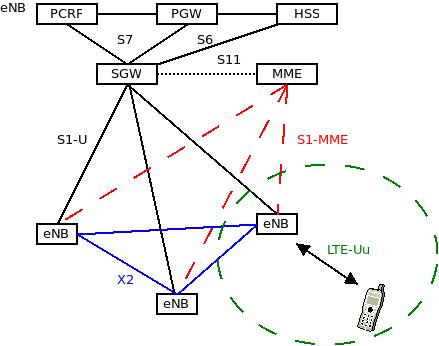
\includegraphics[width=0.7\textwidth]{Imagen/diaLTE.jpg}
			\caption{Arquitectura de la red LTE}
		\end{figure}
		\begin{itemize}
			\item e-NodeB Se ocupa de la gestión de los recursos radio, control de interferencias, compresión de cabeceras IP, cifrado y proteccion de la integridad de datos de usuario, selección del MME y el encaminamiento hacia el S-GW.
			\item Entidades Evolved Packet Core (EPC)
			\begin{itemize}
				\item Mobility Management Entity (MME) Se ocupa del control de acceso, gestión del área de tracking y paging, itinerancia, autentificación y gestiona la selección tanto de S-GW como de P-GW.
				\item Serving Gateway (S-GW) Es la entidad que se ocupa del encaminamiento de paquetes, los niveles de QoS. Cada móvil solo podrá estar conectado a una única S-GW al mismo tiempo.
				\item PDN Gateway (P-GW)
			\end{itemize}
			\item Home Suscriber Server
			\item Policy \& Charging Rules Function
		\end{itemize}
	% subsubsection arquiLTE (end)
% subsection LTE (end)